\documentclass{article}
\usepackage[utf8]{inputenc}
\usepackage{indentfirst}
% The ams packages are required to insert any mathematical symbols that you may require
\usepackage{amsfonts}
\usepackage{amssymb}
\usepackage{amsmath}
\usepackage{amsthm}
% This package is used for embedding things like PDFs and JPEGs into your document
\usepackage{graphicx}
% This package is used for drawing pictures (such as trees)
\usepackage{tikz}
% These packages are used for adding pseudo-code to your document
\usepackage{algorithm}
\usepackage{algorithmic}
% This package is for if you require an appendix
\usepackage{appendix}
\usepackage{ upgreek }

\usepackage{hyperref}

\title{Image Processing \& Computer Vision}
\author{Matt Bessey, Jack Mat, Callum Muir \& Drum Ogilvie}
\date{May 2013}

\begin{document}

\maketitle

\section{Exam Notes}
    Referenced papers detailed content are not examinable. Follow the lab worksheets, they are the best resource.
    
    Understanding the principles and applying skills is more important than memorising equations.
    
    The exam format is two compulsory questions, with 30 marks per question, and two parts per question.

\section{Image Acquisition}
    \subsection{The Dirac-Delta Function}
        What is an image? We can define it as a continuous function $f$ that maps coordinates to colour values. Those coordinates can be in $N$ dimensions

        Dirac Delta Function is a function to sample one point from a continuous image, with the idea being that we combine points to create a whole discrete (pixel) image. This is the ideal capture system, with no point spread or bleeding.
        
        Problem is that optical capture systems (whether an eye or a camera) are never ideal i.e points are blurry and bleed into each other. No big deal, though, because...

    
    \subsection{Representation \& Sampling}
        We have to store images as pixels, which are essentially samples across the continuous 2D image. If we think of each image as a bunch of waves of colour/intensity/luminance in various directions then there will be a highest-frequency wave. We sample at twice the frequency of this wave, and that is the minimum we need to represent the image completely. This frequency is known as the \textbf{Nyquist rate}.
        A way I like to think about it is that if we had a picture full of stripes each 1cm wide, then we can think of the image as a wave of 2cm in length. So we need a pixel in every 1cm, or for each colour of stripe.
        Bad sampling leads to aliasing, which is where images look (as the uninitiated normal people who don't do IPCV would say) ``pixelated''.

\section{Transforms}

    \subsection{Fourier Space}    
        Gives a representation of an image (in the time domain) in the frequency domain. Low levels of detail, or slowly changing gradients, are represented by high magnitudes in the low frequency spectrum. Rapidly changing features, like stripes, are represented by high magnitudes in the high frequency spectrum.
        
        There is only ever one way of showing an image as a combination of waves, so changes in the Fourier space will affect the image in spatial domain.
        
        We can easily convert between spatial and Fourier domain, losslessly. This is known as the Fourier transform and inverse Fourier transform. Commonly implemented as Fast Fourier Transforms - ``FFTs''.
        
        Lines in the Fourier magnitude space correlate to perpendicular lines in the original image. The Fourier space is typically re-centred so that the closer to the origin of the Fourier space we get, the lower the frequency of the waveform that the magnitude at this point represents. We don't need to know the mechanism behind re-centring the 4 quadrants.
        
        The Fourier phase space relates the magnitude space variations to spatial offsets, so the phase space gives a structure of an image, where the magnitude gives the contrast. If you randomise the magnitude space, but keep the phase space, you can usually make out some details from the original image.
        
        This course doesn't really do anything with the phase information. So fear not. Filters that use the magnitude space include high-, low- and band-pass filters; low-pass $\approx$ blurring/smoothing, high-pass $\approx$ sharpening and band-pass filters combine a low and high pass filter to filter all frequencies besides a specific band.
        
        If we smooth the gradient of a filter the effects become more subtle; less artifacts are present in the spatial domain. 
    
    \subsection{Convolution Theorem}
        Convolution in the spatial domain is equivalent to point-wise multiplication in frequency domain, and vice-versa. We will focus on spatial domain convolution. It can be used to perform general operations to a whole image; examples of this include Wiener Deconvolution and sharpening/blurring kernels. A Gaussian blur can be implemented by 2D convolution with an odd-square kernel (3x3, 5x5 etc) which evenly distributes the values across neighbouring pixels. A 3x3 example is here:
        
        $$\begin{bmatrix}
            \frac{1}{9} & \frac{1}{9} & \frac{1}{9} \\[0.4em]
            \frac{1}{9} & \frac{1}{9} & \frac{1}{9} \\[0.4em]
            \frac{1}{9} & \frac{1}{9} & \frac{1}{9}
        \end{bmatrix}$$

        We can restore hidden data by convolving an image with the inverse of the process it has undergone. I.e. if we know the damage that has been done, we can somewhat restore the image. It is important to realise, though, that it's not simply a case of inverting the kernel matrix, because there's no guarantee of invertibility. Reverse kernels usually make sense when you look at them though; For example, a kernel that might mostly fix the blur above would look like this:
        
        $$\begin{bmatrix}
            -1 & -1 & -1 \\[0.1em]
            -1 & 9 & -1 \\[0.1em]
            -1 & -1 & -1
        \end{bmatrix}$$

\section{Edges \& Shapes}
    \subsection{Edge Detection}
        An edge is characterised by a sharp change of image brightness. To find edges, we measure the change of brightness in an image, through differentiation with respect to $x$ and $y$. The gradient gives us the change and it’s normal gives the direction of the change. The edge direction and gradient are always orthogonal to one another.
        
        One approach is convolution. Sobel is a commonly used convolution kernel for this. It uses two kernels, one for change in $x$, and one for change in $y$, here they are, respectively:
        
            $$\begin{bmatrix}
                1 & 0 & -1 \\[0.1em]
                2 & 0 & -2 \\[0.1em]
                1 & 0 & -1
            \end{bmatrix}
            \begin{bmatrix}
                1 & 2 & 1 \\[0.1em]
                0 & 0 & 0 \\[0.1em]
                -1 & -2 & -1
            \end{bmatrix}$$
            
        Before using it, it is a good idea to first perform Gaussian blur to reduce noise. 
        
        To use it, convolve the two kernels with the image. To combine the two results into the gradient magnitude, we use the formula:
        
        $$\mathbf{G} = \sqrt{ {\mathbf{G}_x}^2 + {\mathbf{G}_y}^2 }$$
        
        Where $G_x$ and $G_y$ are the gradients in $x$ and $y$ respectively.
    
    We can also get the edge direction, $\psi$, by the following formula:
    $$
        \psi = arctan\Big(\frac{\mathbf{G_{y}}}{\mathbf{G_{x}}}\Big)
    $$
    
    Note that this vector is tangent to the edge, so the actual gradient occurs perpendicular to it, or at $\psi$ minus $\frac{\pi}{2}$ radians.
    
    \subsection{Line Representation}
    % TODO: This could use a lot of improvement. - Matt
    Any straight line in 2D space can be represented by: 
    
    $$\rho = x \cos \theta+y\sin \theta$$
    
    Where $\rho$ is the orthogonal distance between the line and the origin and $\theta$ is the angle from the positive X axis which is orthogonal to the line. It sounds horrible, but this figure should make it clear. The image on the left is a line in the image space, and the image on the right is the corresponding Hough space point.
    
    \begin{figure}[h]
        \centering
        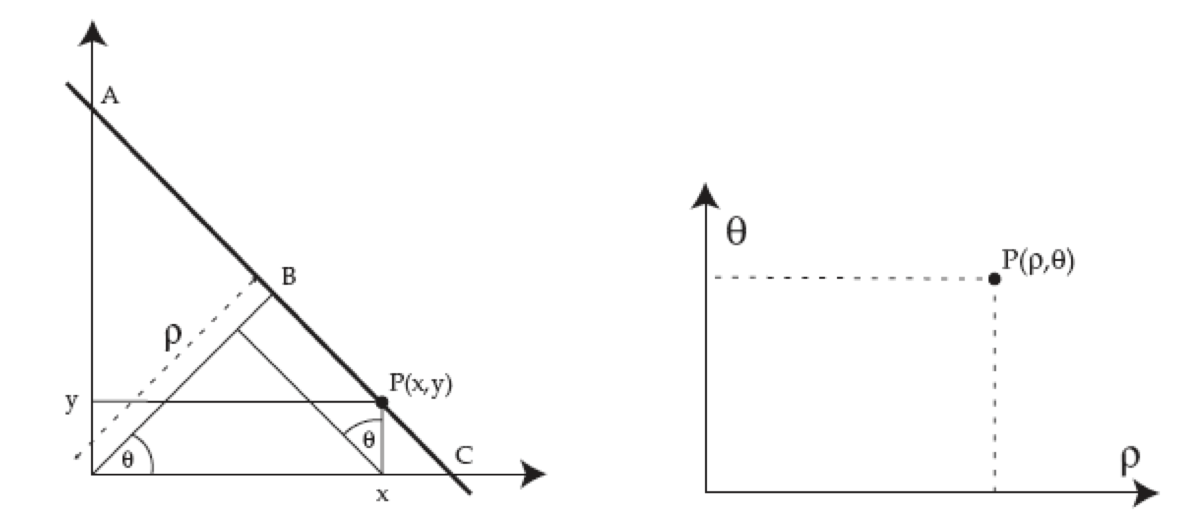
\includegraphics[scale=0.2]{images/linerep.png}
        \caption{Gotta love lines with angles and stuff on them}
    \end{figure}
    
    This is known as the Hough space. The reason we use this representation is that we can easily encode all possible straight lines with only 2 parameters, whereas other encodings either use more parameters or cannot encode certain lines (like how $y = mx + c$ cannot encode vertical lines, for example).
    
    A single point in the image is transformed into a sinusoidal line in the Hough space. The transform itself is hopefully not going to come up, but is available in lecture 4, slide 14.
    
    When detecting lines in an image with this method, you would first detect edge pixels, and increment the Hough space based on only these edge pixels.
    
    Whilst doing it naively (considering all lines that could go through a pixel) is expensive, we can take into account the edge direction of the pixel in order to reduce the number of calculations; only increment lines in the Hough space approximately aligned with the pixel’s edge direction. This means you will not transform to a full sinusoid; instead you will end up incrementing a counter in just a handful of points.
    
    Where strong lines exist in an image, many of the sinusoids / counters will intersect, so you can threshold the hough space to find the peaks, which represent unique lines within the image.
    
    \subsection{Circles}
        Circles are represented in the same way as lines, but with a 3rd dimension for the radius of the circle. Recall from the coursework that the process is to assume different radius sizes, perform the Hough transform for each, and then use the \emph{extremist} extrema (brightest points) to pick the correct radius. For each edge pixel we increment possible centre pixels on both side of it, because we cannot be certain which edge is inside the circle on just one pixel.
    
    \subsection{Generalised Hough Transform}
    
        The generalised Hough transform allows us to specify arbitrary shapes in the Hough space. We can think of a shape as a collection of lines with a `centre of mass', you see, which is really handy. We look at the edge pixels, and for each edge pixel we calculate a vector to the centre of mass, storing it's magnitude and angle from the positive X axis. Having done this for all the edge pixels, we can organise our list based on the edge-direction of the pixel, and eliminate any duplicates. An example of a table and image can be found in Lecture 4, slide 22.
    
    Decoding these is a bit fiddly, but is made fairly simple if you assume that the origin is the centre of mass and work outwards from it.

\section{Segmentation}

    The purpose of segmentation is to understand clusters of an image as recognisable objects. Clusters not necessarily significantly visually distinct. It is beneficial for both simplification of an image, and higher level object description.
    
    Issues: under / over segmentation. Merging two objects into one or splitting one object into multiple.
        
    \subsection{Thresholding}
        Only a useful segmentation method when sufficient contrast exists between segments. Another issue is, how do we choose suitable threshold? For this, a histogram can be helpful. A histogram tells us the distribution of pixel intensities in an image, with spatial data eliminated.
        \subsubsection{Global Threshold Selection}
            Pick an initial threshold estimate in the histogram (a good starting point might be the centre), compute mean for both the sections $m1$ and $m2$, lastly compute the new threshold estimate based on the mean of the two means: $(m1 + m2)/2$. Repeat until convergence.
        \subsubsection{Adaptive Thresholding}
            An alternative approach. We take into account only a local region, by subdividing the image, while applying the above approach. This method handles gradients well.

    \subsection {Edge Based Segmentation}
        Detect strong edges, and extend them by finding weak edges between them, or delete them if we find none, to create closed boundaries around segments.
        \subsubsection{Edge Relaxation}
            Divide and conquer, then expand with confidence. Start by finding all strong edges. Now with each weak edge, decide how to treat them based on the following process:
            \begin{enumerate}
                \item If they have no neighbours, discard.
                \item If they have a single neighbour at one end, do nothing.
                \item If they have two neighbours at one end, decrease their value (as this would make corner off of which they are hanging)
                \item If they have one neighbour at either end, increase their value (as they are the bridge between two strong edges, i.e. the continuation of a line.
                \item If they have more then one neighbour on one end, and exactly one neighbour at the other, increase their value (as they are the intersection of a set of edges).
            \end{enumerate}
        
        When this is done, assume all edges with values above a given threshold are valid edges. KABOOM, BABY!\footnote{That's a Starcraft 2 reference. Just so you know.}
    \subsection{Region Based Segmentation}
        \subsubsection{Region Growing}
            Start with initial seed (a point on the image) and grow area if surrounding pixels satisfy a homogeneity condition. At the point no neighbouring pixels satisfy the condition, pick another seed. Continue this process till all pixels are accounted for.
            
            A homogeneity condition is defined as a mapping of the current region, and its parameters, to a binary decision on a candidate pixel. An example homogeneity condition might be ``the candidate pixel must have an intensity value within 50
            of the region's mean intensity value'', but could be anything that meets the previous definition.
            
        \subsubsection{Split \& Merge}
            Divide and conquer method. The process is to start with 1 large region encompassing the entire image. If the region is not homogeneous (that is to say there is a high variance in the histogram, for example), we split into 4. This process is repeated recursively, and when complete, all touching homogeneous sub-regions are merged together.
            
        \subsubsection{Clustering}
            We perform clustering through, say, K-means, in RGB space, then map back to pixel space.
        
            K-means involves initialising K points in our sample space, and naïvely divide the dataset based on these points. We then calculate the mean value for the points in the dataset, and use these as our new K centres for our clusters. Repeat this process until new means converge on previous means.
            
            K-means is vulnerable to sub-optimal initialisation. One solution to this is to run multiple rounds of K-means, taking the median of means. This reduces the chance of an incorrect solution.

\section{Object Recognition}

    \subsection{Viola \& Jones' Method}
    
        First real-time face detection method. Inventors of Haar-like features. Pretty cool stuff.
    
        \subsubsection{Haar-like Features}
        
            A Haar-like feature considers adjacent rectangular regions at a specific location in a detection window, sums up the pixel intensities in each region and calculates the difference between these sums. This difference is then used to categorise subsections of an image. Simply put, it detects adjacent regions of contrasting intensity of a given size and orientation (regions are always quadrilateral in shape, and can be different in area but they must)
            
            These features are weak classifiers and so many different features are needed for a strong classification. In the Viola–Jones object detection framework, the Haar-like features are therefore Boosted to form a strong learner or classifier.
            
        \subsubsection{Integral Images}
            Also known as a ``summed area table'', it is an efficient data structure to aid in the calculations of sums of a subsection of a grid, or in this case image.
            
            The data structure is simply an $n*m$ matrix (where $n$ and $m$ are the width and height of the image), where each cell holds the sum of all cells above and to the left, plus this cell's value.

        \subsubsection{``BlockImage'' Convolution}
            To get the sum of an area in an image, with top left coordinate, or shift vector, $t(x,y)$ and width/height, or scaling vector $s(x,y)$, we use the integral image as follows:
            
            \begin{enumerate}
                \item Take the value at $(tx+sx,ty+sy)$ (the bottom right coordinate)
                \item Subtract the value at $(tx,ty + sy)$ (the bottom left coordinate's outside neighbour).
                \item Subtract the value at $(tx + sx,ty-1)$ (the top right coordinate's outside neighbour).
                \item Add the value at $(tx-1,ty-1)$ (the top left coordinate's outside neighbour, because we have effectively subtracted this area twice since it intersects the other two rectangles).
            \end{enumerate}
            
            The optimised Haar-like feature algorithm uses this process to sum the black and white rectangle areas, and then subtract one from the other, in a mere 5 steps per rectangle, instead of $O(nxy)$, where $n$ is the number of rectangles.
                        
    \subsection{Boosting \& the AdaBoost algorithm}
        Boosting allows us to easily form a strong classifier from a large number of weak classifiers. This is done by adjusting the weighting of training data over a series of iterations, reducing the overall error. It is best explained as a process of steps, so I shall. While its doubtful you need to remember the exact equations I have included them just in case. Imagine a booster, which runs over $T$ iterations,
        
        \begin{enumerate}
            \item Initialise the weight of every training item to $\frac{1}{m}$
            \item Create a new weak learner, $h_t$
            \item Train this learner on the weighted data to minimise its error\footnote{This simply means, train each classifier this one is made up of, with the weighted data. E.g. in a Bayesian filter we can weight a word by pretending there are more occurences than there are.}, $E_t$.
            \item Computer the importance of this meta-classifier with the formula:
                $$ \alpha_t = \frac{1}{2} \ln{\left (\frac{1-E_t}{E_t}\right )}$$
            \item \textbf{Increase} the weights of \textbf{incorrectly} classified items.
            \item \textbf{Decrease} the weights of \textbf{correctly} classified items.
            \item If $t < T$ GOTO 2.
            \item Our actual classification is now calculated as the sum of each weighted classifier:
                $$ H(x) = \sum\limits_{t=1}^T \alpha_t h_t(x) $$
        \end{enumerate}

\section{Motion}
    \subsection{Perspective Projection}
        Rigid objects can only do two things in this space: rotate, and translate.
        Rotation described as a 3x3 matrix; $R = Rx Ry Rz$. Not dependent on scene depth.
        Translation described as a 3x1 matrix. Dependent on scene depth (focal length) to calculate new position / distance travelled.
        So projecting 3D points onto a 2D image plane leaves us with a 2D motion field.
        
        \begin{tabbing}
            $P(X,Y,Z)$ \quad \= a 3D point in space.\\
            $p(x,y,f)$ \> a point on the image plane.\\
            $O$ \> the camera origin in space.\\
            $o$ \> the camera origin on the image plane.\\
            $f$ \> the focal length of the camera; the distance between $O$ and $o$.\\
            $Z$ \> the optical axis, which starts at $O$ and passes through $o$.\\
        \end{tabbing}
        
        We can project a 3D point in space onto the image plane using the similar triangles formula:   
        
        $$ x = \frac{fX}{Z} $$ $$ y = \frac{fY}{Z} $$
    
    \subsection{Motion Field}
        Unlike the optic flow field, the motion field is not based on the appearance of the scene, but purely depth data, a good way to think of this is how a Kinect sees the world; if you moved a flat plane laterally past the camera, it would not affect the motion field, because in depth terms nothing has occurred. 
    
        2D Motion Field Equation:
        
        $$ v_x = (fT_X - xT_Z)/Z + f\theta _Y - \theta_Z y - (\theta_Xxy-\theta_Yx^2)/f $$
        $$ v_y = (fT_Y - yT_Z)/Z + f\theta _X - \theta_Z x - (\theta_Yxy-\theta_Xx^2)/f $$
        
        Terrifying right? Lets break it down a little. We're already familiar with most of what we see here. $T_{X/Y/Z}$ and $\theta_{X/Y/Z}$ are new, but don't worry, those are just the angular and rectilinear velocity of the point. These are used to calculate the rotation and translation matrix in the Stereo section. While these equations are a bitch to remember, the key thing to note is that rotation and translation aren't strongly connected, so if a question specifies solely a translation, or rotation, that's half the equation eliminated already.

    \subsection{Optical Flow}
        Model: For a $2D+t$ dimensional case a voxel (a 3D pixel) at location $(x,y,t)$ with intensity $I(x,y,t)$ will have moved by $\Delta x$, $\Delta y$ and $\Delta t$ between the two image frames, and the following ``image constraint equation'' can be given: 
        $$I(x,y,t) = I(x+\Delta x, y + \Delta y, t + \Delta t)$$
        Which in words reads as, for every voxel at time $t$, there is a voxel at time $t + \Delta t$ with offset $\Delta x, \Delta y$ that corresponds to the original voxel. We \emph{love} this shit because with the help of some other assumptions it allows us to express mathematically the motion in the scene between two frames, based on the difference in luminosity. In words, between two frames along the motion trajectory, luminosity does not change. Or in maths: 
            
        $$ \frac{\partial I}{\partial x}V_x+\frac{\partial I}{\partial y}V_y+\frac{\partial I}{\partial t} = 0 $$
        
        \emph{Note, Andrew likes to substitute the partial derivatives with $E_x$, $E_y$, and $E_t$.}
        
        Unfortunately, both $V_x$ and $V_y$ are unknown, and since they are orthogonal to one another, we cannot infer anything about one from the other, so \textbf{the equation has no single solution}. This is why we have to add extra constraints onto the problem in order to solve it. An excellent example of this is the Lucas-Kanade method which we will discuss in a jiffy.
    
    \subsection{Aperture Problem}
        % Is this simply another way of explaining what I said above? - Matt
        When only looking at pixels in a small area, the direction of movement is ambiguous. E.g. the side edge of an object may appear static when the object as a whole is moving forward. This is known as the aperture problem. The OFE is victim to this problem, and only by assuming certain conditions, can we use it to estimate motion.
        
    \subsection{Motion Estimation: Lucas \& Kanade method}
        Based on optical flow estimation. The Lucas \& Kanade method assumes that $V_x$ and $V_y$ are constant (or near constant) within a local area. This assumption means for a local area of $n$ pixels, we now have $n$ equations sharing two unknowns. Suddenly our unsolvable equation has become very much solvable!
        
        The only remaining issue is that in practice, velocity is \emph{not} constant within a local area, and even if it was, noise will make it not appear so, meaning our simultaneous equations have no solution. To solve this, we solve the equation using the least squares approach; we find the velocity that gives the smallest sum error across the $n$ samples.
        
\section{Stereo}
    Stereo vision allows us to extract 3D structure from two (or more) images taken from different viewpoints. The position of an object in each image depends on its depth, it is an inverse relationship. The disparity increases as the depth decreases. There are 3 steps to perform successful stereo positioning. Calibration; finding the relative position of two cameras. Correspondence; determining matching points in the stereo views. Reconstruction; determining 3D location of matched points via triangulation.
        
    \subsection{Epipolar Geometry}
        \subsubsection{Maths}
        \begin{center}
            \begin{tabular}{l p{10cm}}
                $p$ & A point in the 2D image. \\
                
                $P$ & A 3D point in space. \\
                
                $T$ & The Translation matrix. Defines the translation from one camera to the other. \\
                
                $R$ & The Rotation matrix. Defines the rotation from one camera to the other. \\
                
                $P_l = R_tP_r + T$ & Position of a point in the right camera's view, in the left. \\
                $P_r = R(P_l - T)$ & Position of a point in the left camera's view, in the right. \\
                
                $S$ & The cross product of the Translation matrix. \\
                
                $E = RS$ & The Essential matrix. Holds the important property of $P_R^T E P_L = 0$. The essential matrix gives us a relationship between points in the left and right image plane. \\
                
                $F = M^T_R E M_L$ & The Fundamental matrix. Holds the same properties as the Essential matrix,  but for pixel coordinates rather than real world. \\
                
                $M_R$ & The calibration matrix for the right camera. \\

                $u_L = Ep_L$ & Substitution used in epipolar line equations. \\

                $(\hat{x},\hat{y})$ & Pixel image plane coordinates. \\
                
                $(x,y)$ & Real world image plane coordinates. \\


            \end{tabular}
        \end{center}

        \subsubsection{Epipolar Lines}
            Imagine we have two cameras whom we know the position of, both looking at a point $P$ in 3D space. We draw a line from the origin of these cameras, to the point, and then project each camera's line onto the other's image plane. These are epipolar lines.
            
            What an epipolar line tells us is that if we find a point in one camera, it must lay somewhere along the epipolar line seen in the other camera. This information is useful in stereo when looking for key points. The equation for an epipolar line in the right image, based on a point in the left, is $p^T_Ru_L = 0$. Expanded this is:

            $$x_Ru_{L1} + y_Ru_{L2} + fu_{L3} = 0$$
            
        \subsubsection{Triangulation}
            The process can also be reversed; when we know the relative position of the cameras, it is possible to plot a point seen by both cameras in 3D space through triangulation. In practice it is impossible to have perfectly calibrated cameras where each pixel corresponds exactly to a pixel in the other camera, such that their epipolar lines perfectly intersect. However, we can find the closest point between them by finding the intersecting line orthogonal to both lines, (but we do not need to be able to do this).
            
    \subsection{Harris Corners}
    
        The Harris corner algorithm is a salient point detection algorithm. It detects corners by looking for a sharp difference in gradient within a local area. This works because at a corner, the gradient of an edge rotates by 90 degrees.
            

    \subsection{RANSAC}
        RANdom SAmple Consensus: Method of calculating the fundamental matrix $F$, based on a scene containing unknown geometry. Useful for getting rid of outliers in a region based matching scheme.
Good 2D example:
        
        \url{http://visual-experiments.com/demo/ransac.js}
        
        Process: 
        \begin{enumerate}
            \item Build a set of all possible salient (key) points, through another algorithm, say SIFT.
            \item Randomly select a subset from this set.
            \item Compute $F$ based on this subset.
            \item Assess computed $F$ based on the rest of the set\footnote{In this sense it's a bit like 10-fold cross validation, from Machine Learning}.
            \item Repeat until $F$ is within a set error bound.
        \end{enumerate}

    \subsection{SIFT}
        The Scale Invariant Feature Transform detects key points, also known as salient points, in an image. Scale invariant meaning that the camera can zoom in (or scale) without matching issues. The process we use is to Gaussian blur the image to different levels and look at the difference between adjacent levels. Creating a Difference of Gaussian or DoG tree.

        We then create spatial gradient descriptor (vector) for each extrema in the DoG tree, or in other words, a descriptor of each point with a large difference between the two Gaussians. The descriptor is a 128D vector, composed of a 4x4 blocks, each containing an 8 bin orientation histogram. Each histogram therefore describes the magnitude of the intensity gradient in 45$^\circ$ intervals. This approach is so powerful because comparing descriptors is achieved simply by comparing the Euclidean distance between them. We can compare the descriptors between two images to find matching points in the two images.

        It is the multiple levels of Gaussian blur that make the system scale invariant. By finding key points at high blur values, we find good key points for detection far away. The drawback is sparse results; the algorithm only finds specific points in the scene. It can be used with RANSAC to compute $F$ though.

\end{document}
